% This is "sig-alternate.tex" V2.1 April 2013
% This file should be compiled with V2.5 of "sig-alternate.cls" May 2012
%
% This example file demonstrates the use of the 'sig-alternate.cls'
% V2.5 LaTeX2e document class file. It is for those submitting
% articles to ACM Conference Proceedings WHO DO NOT WISH TO
% STRICTLY ADHERE TO THE SIGS (PUBS-BOARD-ENDORSED) STYLE.
% The 'sig-alternate.cls' file will produce a similar-looking,
% albeit, 'tighter' paper resulting in, invariably, fewer pages.
%
% ----------------------------------------------------------------------------------------------------------------
% This .tex file (and associated .cls V2.5) produces:
%       1) The Permission Statement
%       2) The Conference (location) Info information
%       3) The Copyright Line with ACM data
%       4) NO page numbers
%
% as against the acm_proc_article-sp.cls file which
% DOES NOT produce 1) thru' 3) above.
%
% Using 'sig-alternate.cls' you have control, however, from within
% the source .tex file, over both the CopyrightYear
% (defaulted to 200X) and the ACM Copyright Data
% (defaulted to X-XXXXX-XX-X/XX/XX).
% e.g.
% \CopyrightYear{2007} will cause 2007 to appear in the copyright line.
% \crdata{0-12345-67-8/90/12} will cause 0-12345-67-8/90/12 to appear in the copyright line.
%
% ---------------------------------------------------------------------------------------------------------------
% This .tex source is an example which *does* use
% the .bib file (from which the .bbl file % is produced).
% REMEMBER HOWEVER: After having produced the .bbl file,
% and prior to final submission, you *NEED* to 'insert'
% your .bbl file into your source .tex file so as to provide
% ONE 'self-contained' source file.
%
% ================= IF YOU HAVE QUESTIONS =======================
% Questions regarding the SIGS styles, SIGS policies and
% procedures, Conferences etc. should be sent to
% Adrienne Griscti (griscti@acm.org)
%
% Technical questions _only_ to
% Gerald Murray (murray@hq.acm.org)
% ===============================================================
%
% For tracking purposes - this is V2.0 - May 2012
\newcommand{\refalg}[1]{Algorithm~\ref{#1}}
\newcommand{\refsec}[1]{Sect.~\ref{#1}}
\newcommand{\reffig}[1]{Fig.~\ref{#1}}
\newcommand{\refsubfig}[1]{Fig.~\subref{#1}}
\newcommand{\reftab}[1]{Table~\ref{#1}}
\newcommand{\refeqn}[1]{(\ref{#1})}
\newcommand{\reflst}[1]{Listing~(\ref{#1})}
\newcommand{\bigo}[1]{\mathcal{O}(#1)}

\documentclass{sig-alternate}

\usepackage{subfigure}

\begin{document}

% Copyright
\setcopyright{acmcopyright}
%\setcopyright{acmlicensed}
%\setcopyright{rightsretained}
%\setcopyright{usgov}
%\setcopyright{usgovmixed}
%\setcopyright{cagov}
%\setcopyright{cagovmixed}


% DOI
%\doi{000000} ??????  

% ISBN
%\isbn{000000} ???????

%Conference
\conferenceinfo{EASC '16}{April 26--29, 2016, Stockholm, Sweden}

%\acmPrice{\$15.00}

%
% --- Author Metadata here ---
\conferenceinfo{EASC2016}{'16, Stockholm, Sweden}
%\CopyrightYear{2007} % Allows default copyright year (20XX) to be over-ridden - IF NEED BE.
%\crdata{0-12345-67-8/90/01}  % Allows default copyright data (0-89791-88-6/97/05) to be over-ridden - IF NEED BE.
% --- End of Author Metadata ---

\title{Scaling Behavior of Nek5000}
\subtitle{Subtitle}
%
% You need the command \numberofauthors to handle the 'placement
% and alignment' of the authors beneath the title.
%
% For aesthetic reasons, we recommend 'three authors at a time'
% i.e. three 'name/affiliation blocks' be placed beneath the title.
%
% NOTE: You are NOT restricted in how many 'rows' of
% "name/affiliations" may appear. We just ask that you restrict
% the number of 'columns' to three.
%
% Because of the available 'opening page real-estate'
% we ask you to refrain from putting more than six authors
% (two rows with three columns) beneath the article title.
% More than six makes the first-page appear very cluttered indeed.
%
% Use the \alignauthor commands to handle the names
% and affiliations for an 'aesthetic maximum' of six authors.
% Add names, affiliations, addresses for
% the seventh etc. author(s) as the argument for the
% \additionalauthors command.
% These 'additional authors' will be output/set for you
% without further effort on your part as the last section in
% the body of your article BEFORE References or any Appendices.

\numberofauthors{6} %  in this sample file, there are a *total*
% of EIGHT authors. SIX appear on the 'first-page' (for formatting
% reasons) and the remaining two appear in the \additionalauthors section.
%
\author{
% You can go ahead and credit any number of authors here,
% e.g. one 'row of three' or two rows (consisting of one row of three
% and a second row of one, two or three).
%
% The command \alignauthor (no curly braces needed) should
% precede each author name, affiliation/snail-mail address and
% e-mail address. Additionally, tag each line of
% affiliation/address with \affaddr, and tag the
% e-mail address with \email.
%
% 1st. author
% 1st. author
\alignauthor
Oana Marin\\
       \affaddr{*}\\
       \affaddr{*}\\
       \affaddr{*}\\
       \email{*}
% 2nd. author
\alignauthor
Nicolas Offermans\\
       \affaddr{Linn\'{e} Flow Center}\\
       \affaddr{KTH Mechanics, Royal Institute of Technology}\\
       \affaddr{10044 Stockholm, Sweden}\\
       \email{nof@mech.kth.se}
% 3rd. author
\alignauthor 
Adam Peplinski\\
       \affaddr{*}\\
       \affaddr{*}\\
       \affaddr{*}\\
       \email{*}
\and  % use '\and' if you need 'another row' of author names
% 4th. author
\alignauthor 
Michel Schanen\\
       \affaddr{*}\\
       \affaddr{*}\\
       \affaddr{*}\\
       \email{*}
% 5th. author
\alignauthor 
Philipp Schlatter\\
       \affaddr{*}\\
       \affaddr{*}\\
       \affaddr{*}\\
       \email{*}
% 6th. author
\alignauthor
Jing Gong\\
       \affaddr{PDC-HPC}\\
       \affaddr{KTH, Royal Institute of Technology}\\
       \affaddr{10044 Stockholm, Sweden}\\
       \email{gongjing@kth.se}
}
% There's nothing stopping you putting the seventh, eighth, etc.
% author on the opening page (as the 'third row') but we ask,
% for aesthetic reasons that you place these 'additional authors'
% in the \additional authors block, viz.
%\additionalauthors{Additional authors: John Smith (The Th{\o}rv{\"a}ld Group,
%email: {\texttt{jsmith@affiliation.org}}) and Julius P.~Kumquat
%(The Kumquat Consortium, email: {\texttt{jpkumquat@consortium.net}}).}
\date{21 March 2016}
% Just remember to make sure that the TOTAL number of authors
% is the number that will appear on the first page PLUS the
% number that will appear in the \additionalauthors section.

\maketitle
\begin{abstract}
In this paper, strong scaling and benchmarking of the high-order spectral element solver Nek5000 are performed. The previous extensive benchmarking for Nek5000 was done for terascale computers. This study updates the results to modern computers and assess the ability of the code to run efficiently on the next generation of exascale supercomputers. For several test cases, the main blocks of the code are timed and a sampling tool is use to measure the communication time over a large range of processors. The test cases correspond to a turbulent flow in a straight pipe at four different friction Reynolds numbers $Re_{\tau} = 180$, $360$, $550$ and $1000$. Different architectures are studied, namely IBM Blue Gene/Q, Cray XC40 and Cray XK7 supercomputers. A theoretical model for parallel performance is introduced and compared to the numerical results. We also study the effect of the two coarse grid solvers XXT and AMG on the computational time.
\end{abstract}


% Code generated by the tool at
% http://dl.acm.org/ccs.cfm
%
% I generated what follows quite arbitrarily... Do not hesitate to modify.
% Is it even necessary?
 \begin{CCSXML}
<ccs2012>
<concept>
<concept_id>10010147.10010169.10010170</concept_id>
<concept_desc>Computing methodologies~Parallel algorithms</concept_desc>
<concept_significance>500</concept_significance>
</concept>
<concept>
<concept_id>10010147.10010169.10010170.10010174</concept_id>
<concept_desc>Computing methodologies~Massively parallel algorithms</concept_desc>
<concept_significance>300</concept_significance>
</concept>
<concept>
<concept_id>10003752.10003777.10003780</concept_id>
<concept_desc>Theory of computation~Communication complexity</concept_desc>
<concept_significance>300</concept_significance>
</concept>
<concept>
<concept_id>10010405.10010432</concept_id>
<concept_desc>Applied computing~Physical sciences and engineering</concept_desc>
<concept_significance>300</concept_significance>
</concept>
</ccs2012>
\end{CCSXML}

\ccsdesc[500]{Computing methodologies~Parallel algorithms}
\ccsdesc[300]{Computing methodologies~Massively parallel algorithms}
\ccsdesc[300]{Theory of computation~Communication complexity}
\ccsdesc[300]{Applied computing~Physical sciences and engineering}


%
% End generated code
%

%
%  Use this command to print the description
%
\printccsdesc

% We no longer use \terms command
%\terms{Theory}

\keywords{Nek5000; Scaling; Benchmarking}

\section{Introduction}

The resolution of partial differential equations (PDE) is common practice nowadays in the scientific community. However, developing a code that scales linearly on a large number of cores still remains a challenging task. In this paper, we study the behavior of Nek5000, a solver for fluid mechanics and heat transfer problems, on a large number of processors and assess its ability to run efficiently on the next generation of exascale supercomputers. Cite\cite{fischer:scaling} and \cite{tufo:terascale}...

\subsection{Hardware}

The test cases were run on three different supercomputers, namely Mira from the Argonne National Laboratory, USA, Titan from the Oak Ridge National Laboratory, USA, and Beskow from the PDC Center for High Performance Computing, KTH, Sweden. A quick overview of the characteristics of each computer is summarized in Table \ref{tab:computer_charac}

% Add other fields to the table?
% Put latency and bandwidth in another table?
\begin{table*}
\centering
\caption{Overview of the characteristics of the different supercomputers.}
\begin{tabular}{l|ccccc} 
\hline
 & Architecture & \# of cores & cores/node & $\alpha$ & $\beta$\\
 \hline
Mira & IBM BG/Q & $786,432$ & $16$ & $5000$ & $5$\\ 
Titan & Cray XK7 & $299,008$ & $16$ & $*$ & $*$\\ 
Beskow & Cray XC40 & $53,632$ & $32$ & $*$ & $*$\\
\hline
\end{tabular}
\label{tab:computer_charac}
\end{table*}

The values for the latency $\alpha$ and the inverse bandwidth $\beta$ have been computed following a "ping-pong" test as described in \cite{fischer:scaling}. During this test, the time required to send and receives messages of various sizes between different processors is measured and values of the latency and bandwidth are deduced.

% Show graph with results of the ping pong test?
% Explain that we took minimum values
% Discuss noise and "randomness" of the results on Cray machines


\section{Prior Work}
Link to the complexities in the Fischer paper -> multiplicities
Explain finite difference link
\section{Nek}

\subsection{Method}
projections

\subsubsection{Splitting method}

We consider the resolution of the Navier-Stokes equations for an incompressible flow and Newtonian fluid
\begin{align}
 \nabla \cdot \mathbf{u} & = 0, \label{eqn:NS_continuity}\\
 \frac{\partial \mathbf{u}}{\partial t} + (\mathbf{u \cdot \nabla}) \mathbf{u} & = - \nabla p + \frac{1}{Re} \nabla^2 \mathbf{u} + \mathbf{f} \label{eqn:NS_momentum},
\end{align}
where $\mathbf{u}$ is the velocity field and $p$ the thermodynamic pressure. The Reynolds number $Re = \frac{U L}{\nu}$ is expressed as a function of a typical velocity scale $U$, length scale $L$ and kinematic viscosity $\nu$. Equations (\ref{eqn:NS_continuity}) and (\ref{eqn:NS_momentum}) are called the continuity and momentum equations respectively. The numerical integration of the momentum equation is done explicitely for the nonliean convective terms and implicitely for the viscous and pressure term according to a scheme developped by A. G. Tomboulides \cite{Tomboulides1997}. This method is referred to as $\mathbb{P}_N\mathbb{P}_N$ and leads to the following system of equations for one iteration
\begin {align}
 \mathbf{F} \left( \mathbf{u}^{n} \right) & = \sum_{j=1}^{k} \frac{-b_j}{\Delta t} \mathbf{u}^{n+1-j} + \sum_{j=1}^{k} a_j N \left( \mathbf{u}^{n+1-j} \right) +  \mathbf{f}^{n+1} \label{eqn:rhs1}\\
 \mathbf{\tilde{F}} \left( \mathbf{u}^{n} \right) & = \mathbf{F}\left(\mathbf{u}^{n}\right) + \mu \sum_{j=1}^{k} a_j \left( \nabla \times \left( \nabla \times \mathbf{u}^{n+1-j} \right) \right) \label{eqn:rhs2} \\
 \Delta p^{n+1} & = \nabla \cdot \left( -\frac{b_0}{\Delta t} \mathbf{u}^{n+1} + \mathbf{\tilde{F}} \left( \mathbf{u}^{n} \right) \right) \label{eqn:hmhz_pres}\\
 \Delta \mathbf{u}^{n+1} & = - \frac{b_0}{\Delta t} \mathbf{u}^{n+1} + \nabla p^{n+1} + \mathbf{F} \left( \mathbf{u}^{n} \right). \label{eqn:hmhz_vel}
\end {align}
The nonlinear terms have been gathered in operator $N \left( \mathbf{u}^{k} \right)$. The coefficients $b_k$ and $a_k$ are the coefficients for the explicit discretization of the time derivative and convective terms.

% \begin{align}
%  \mathbf{u}_i^* & = \beta_0 \mathbf{u}_i^n + \beta_1 \mathbf{u}_i^{n-1} + \beta_2 \mathbf{u}_i^{n-2}, \label{eqn:extrap_vel}\\
%  \mathbf{h}_i^n & = N(\mathbf{u}_i^n) + B \mathbf{f}_i + ???, \label{eqn:rhs}\\
%  A \delta \mathbf{p}^n & = \nabla \cdot \left[ \left( \sum_{i=1}^3 \frac{-1}{Re} (\nabla \times (\nabla \times \mathbf{u}_i^*)) + B^{-1} \mathbf{h}_i^n \right) \right]\nonumber\\
%  & \quad - A \mathbf{p}^n , \label{eqn:hmhz_pres} \\
%  A \delta \mathbf{u}^{n} & = -A \mathbf{u}^{n} + \mathbf{h}_i^n \label{eqn:hmhz_vel},\\
%  \mathbf{p}^{n+1} &= \mathbf{p}^{n} + \mathbf{\delta p}^{n}, \label{eqn:update_p} \\
%  \mathbf{u}_i^{n+1}& = \mathbf{u}_i^{n} + \mathbf{\delta u}_i^{n}.  \label{eqn:update_u} 
% \end{align}
% The operators $A$ and $B$ represent the discrete Laplacian operator and the mass matrix respectively. The index $i=1,2,3$ represents the 3 spatial directions $x$, $y$ and $z$. The intermediate velocity $\mathbf{u}_i^*$ is extrapolated using a third order Adams-Bashforth scheme in Equation (\ref{eqn:extrap_vel}). The corresponding coefficients $\beta_k$ are given by $\beta_0 = \frac{23}{12}$, $\beta_1 = \frac{-4}{3}$ and $\beta_2 = \frac{5}{12}$ (??). The term $\mathbf{h}_i^n$ from equation (\ref{eqn:rhs}) contains the nonlinear convective term $N(\mathbf{u}_i^n)$ evaluated explicitely, the external forcing $\mathbf{f}_i$ and ???. Equation (\ref{eqn:hmhz_pres}) is solved using aGeneralized minimal residual method (GMRES), while equation (\ref{eqn:hmhz_vel}) is solved using the conjugate gradient (CG) mehtod. Furthermore, both the pressure and velocity vectors are projected onto a space of previous solutions in order to speed up the convergence of the iterative solvers. Projections occur before and after the 
% iterative solver. %When solving equations (\ref{eqn:hmhz_pres}) and (\ref{eqn:hmhz_vel}), we obtain the corrections for the pressure and the velocity that we can use to update those variables in Equations \ref{eqn:update_p} and \ref{eqn:update_u}.

%\subsubsection{Coarse grid solver}

% introduce coarse grid solver for the pressure

\subsection{Implementation}
\label{sec:implementation}
\subsubsection{Code structure}
\label{sec:code}

\subsubsection{Instrumentation for the Timers}
\label{sec:timers}
Our strategy for timing the code execution is twofold. For one, we use MPI
timers for the wall clock time and profiling libraries that were deemed suitable
for our use case. We are running the code on our test case (see
\refsec{sec:pipe}) after a full restart for 50 time steps. We save 5 past
projections and are measuring the time from the 30th to the 50th time step; in
total 20 time steps. 
\paragraph{MPI Timers}
Based on the
structure presented in \refsec{sec:code} we placed 9 timers in the code that are
only switched on during the last 20 time steps. Each timer measures the wall
clock time using the MPI timer ({\tt MPI\_Wtime}) followed by a barrier
({\tt MPI\_Barrier}) guaranteeing coherent and synchronized measurements. We
have run the code without synchronization and timers to evaluate the created
overhead due to our measurements. In all instances this overhead has been far
below 5\%. 
Different timers have been placed within the code in order to measure time for the main blocks of the solution. The different timers are
\begin{itemize}
 \item \textit{totaltime}: total time spent for all iterations.
 \item \textit{tmakef}: time to compute $\mathbf{F} \left( \mathbf{u}^{n} \right)$, i.e.\ the right hand side of equation (\ref{eqn:rhs1}).
 \item \textit{tcrespsp}: time to compute the right hand side of equation (\ref{eqn:hmhz_pres}).
 \item \textit{tpresproj1}: time to project the pressure before the iterative solver.
 \item \textit{tpresprojhmhz}: time to solve equation (\ref{eqn:hmhz_pres}).
 \item \textit{tpresproj2}: time to project the pressure after the iterative solver.
 \item \textit{tvproj1}: time to project the velocity before the iterative solver.
 \item \textit{tvprojhmhz}: time to solve equation (\ref{eqn:hmhz_vel}).
 \item \textit{tvproj2}: time to project the velocity after the iterative solver.
 \item \textit{tcoarse}: time for the coarse grid solver for the pressure.
\end{itemize}
\paragraph{Craypat and Hardware Performance Monitor}
In order to measure the time spent in communication we relied on Craypat for
Beskow and Titan and on Hardware Performance Monitor (HPM) for Mira. Both tools
allow us to the total time spent in communication during the targeted 20 time
steps. In addition HPM gives additional information on the cash misses and the load
imbalance.

%\subsection{Models for parallel performance}

%\subsubsection{Computational complexity}

%\subsubsection{Communication model}

% The total time and the time spent in the different parts of the code were computed by measuring the CPU time at appropriate locations in the code. This method is easy to implement, reliable and adds little overhead to the simulations. The measure of the communication time is a trickier task. This is done on Mira using the HPM-sampling tool (? -> add some more info maybe). On the Cray machines, we use the CrayPat performance analysis framework. This tool samples the code during execution at a frequency of $\unit[100]{Hz}$ and reports in which function the sample was found. Then, we assume that the proportion of the total time spent in a given function is equal to the proportion of samples within this function. If the number of samples is large enough, statistics is reliable. Furthermore, it induces a low overhead. A profiling procedure, where all function calls are tracked, could also be used but overhead in time is about $50\%$ and the method is therefore rejected.
% 
% In practice, each simulation is restarted from a previously computed turbulent solution and is run during $50$ time steps. The projections for velocity and pressure are turned on after $5$ time steps, the number of the previous pressure solutions saved is $20$ and the timers are turned on during the last $20$ time steps. Therefore, heavy input/output is not included and projections are working fully during the measurement period.

% Present system of equations
% Describe briefly the algorithm behind nek
% Mention and discuss PN-PN
% Discuss the two coarse grid solver XXT and AMG

\section{Performance and Scaling Analysis}
\label{sec:analysis}
Notes: c32
Large scale runtime performance is influenced by 
\begin{enumerate}
  \item Network topology
  \item Time $T_a$ and $T_c$ spent in computation and communication,
    %respectively
  \item ratio of runtime and communication times: $r \leq \dfrac{T_a}{T_c}$,
  \item degrees of freedom $N$ per process $P$: $\dfrac{N}{P}$,
  \item partitioning imbalance.
\end{enumerate}

We will measure the load imbalance, cache misses, multiplicities of grid points
across as well as weak and strong scaling.
While relying on the results of \cite{tufo:terascale}, we want in particular to verify
experimentally the strong scaling limit which is defined as the ratio of $\dfrac{N}{P}$ where
$\dfrac{T_a}{T_c}\leq 1$ inequality is equal to $1$ with increasing $P$. The
abstraction of communication and computation time does not take into account
factors as load imbalance, cache misses or accelerated collective communications.

The communication is subdivided into nearest neighbour (NN) and so called
allreductions. As the NN hints, the communication takes place between a spacial
partition and all of its neighbours. In a 3D cubic with cubic partitioning this
would be 8 for the vertices, 4 for the edges and 2 for the faces. We assume that
all NN on mesh are also nearest neighbours on the partitioning mapped to the
physical topology of the hardware. We will prove in \refsec{sec:abstractions}
that our use case presented in the next section is equivalent to a cubic
partitioning and rely on the complexities of \cite{fischer:scaling} for $T_c$ and
$T_a$. The performance of allreduce is a core indicator of a system's
performance and is dependent on its network hardware. The most prevalent
complexities for allreductions are given by $\bigo{\dfrac{n}{P}\cdot log(P)}$. All
systems used in this paper rely on accelerated allreduce MPI communication that have
a complexity of $\bigo{O(n)}$, independently of $P$. Beskow uses the dragonfly
topology where accelerated collectives are being presented in
\cite{jain2012collectives}. Titan and Mira use a 3D and 5D torus, getting the
reduction cost down to $\alpha \cdot c \cdot n$ where $c$ is a low constant
value. In the end, the collective communication is the dominant and
differentiating factor in the scaling behavior of Nek on those three systems.

A generic case, widely known across the CFD community, is used to explore the
scaling behavior of Nek. This should allow potential users to estimate and
compare the scaling of Nek to other CFD software.
\subsection{Test Case: Pipe}
\label{sec:pipe}

The test case considered is the turbulent flow in a straight pipe. A thorough description of the flow configuration as well as a detailed analysis of the physical results can be found in \cite{Khoury2013}. The flow was run at four different friction Reynolds numbers $Re_{\tau} = 180$, $360$, $550$ and $1000$. A summary of the different simulations and associated number of elements and number of grid points is presented in Table \ref{tab:pipe_conf}. The friction Reynolds number is defined as $Re_{\tau} = u_{\tau} R / \nu$, where $u_{\tau}$ is the friction velocity $R$ is the radius of the pipe and  $\nu$ is the kinematic viscosity. The bulk Reynolds number is defined as $Re_{b} = 2 U_b R / \nu$, where $U_b$ is the mean bulk velocity. 

\begin{table}
\centering
\caption{Summary of the different pipe flows configurations.}
\begin{tabular}{llrr} 
\hline
$Re_{\tau}$&$Re_{b}$&\# of elements & \# of grid points\\ 
\hline
$180$ & $5300$ & $36,480$ & $18.67 \times 10^6$\\
$360$ & $11,700$ & $237,120$ & $121.4 \times 10^6$\\ 
$550$ & $19,000$ & $823,632$ & $437.0 \times 10^6$\\ 
$1000$ & $37,700$ & $1,264,032$ & $2.184 \times 10^9$\\
\hline
\end{tabular}
\label{tab:pipe_conf}
\end{table}
%\subsection{Abstractions and Assumptions}
%\label{sec:abstractions}
%\subsubsection{$\alpha$, $\beta$}
%\subsubsection{Imbalance}
%\subsubsection{Weak/Strong Scaling, Efficiency}
%\subsubsection{Cache Misses and Scaling}
%\subsubsection{Partitioning and Imbalance}


\section{Results}

Our four test cases were run with various processor counts on three systems. The
lower bound for the processor count is given by the amount of RAM to fit a given
problem into memory. Nek5000 has roughly a memory requirement of 500 fields
times the number of degrees of freedoms. The upper bound was either due to the
administrative limit of getting access to the maximum number of processors
(Beskow and Titan) or by the limit of having 1 or 2 elements per process. As has
been pointed out in \refsec{sec:code}, the parallelization of Nek5000 is at the
element level so that one element may not be partitioned further. 
As anticipated in \refsec{sec:timers}, we measure the communication time and
computation time of the chosen 20 timesteps. 

In \cite{fischer:scaling} the point where $r=\dfrac{T_a}{T_c}=1$ was estimated
to be at about $\frac{n}{P}=2000$ for the conjugent gradient (CG) and $20000$ or
$7000$ (BG/Q) for the algebraic multigrid (AMG). As described in \refsec{sec:code}, the
Nek5000 solvers XXT and PNPN consist of several CG and AMG solves. Furthermore,
there is an overhead for the setup, the projections, the coarse solve and other
none runtime relevant components. Moreoever, the convergence of the underlying
algorithms is also very case dependent, thus influencing the overall runtime
behavior. Our runtimes give an overall impression of the Nek5000 behaviour on
various systems based on a generic well known case in CFD (see
\refsec{sec:pipe}). 

The scaling plots for all three
systems in \reffig{fig:mira} and \reffig{fig:beskow} are the fundamental
measurements for our further analysis of the weak/strong scaling, computation
versus communication time and load imbalance.
\begin{figure}
  \centering
  \subfigure[ReTau180 Mira]{
  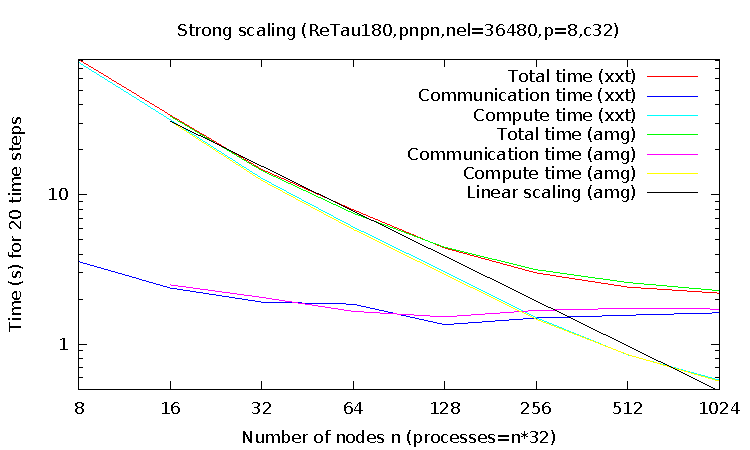
\includegraphics[width=\linewidth]{./figures/mira/scaling_ReTau180.pdf}
  }
  \subfigure[ReTau360 Mira]{
  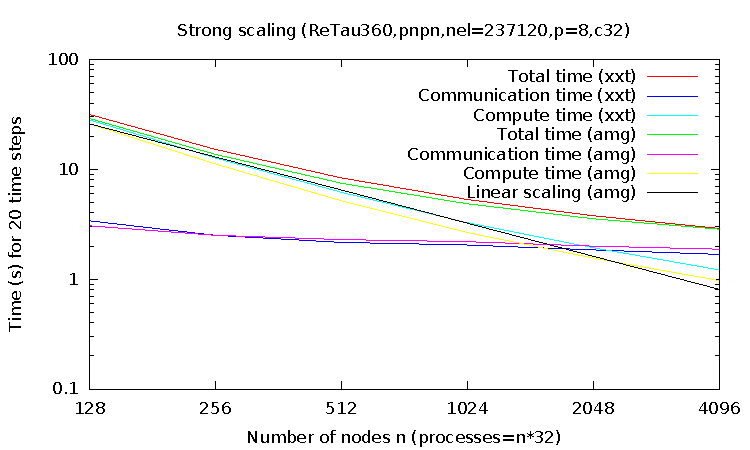
\includegraphics[width=\linewidth]{./figures/mira/scaling_ReTau360.pdf}
  }
  \subfigure[ReTau550 Mira]{
  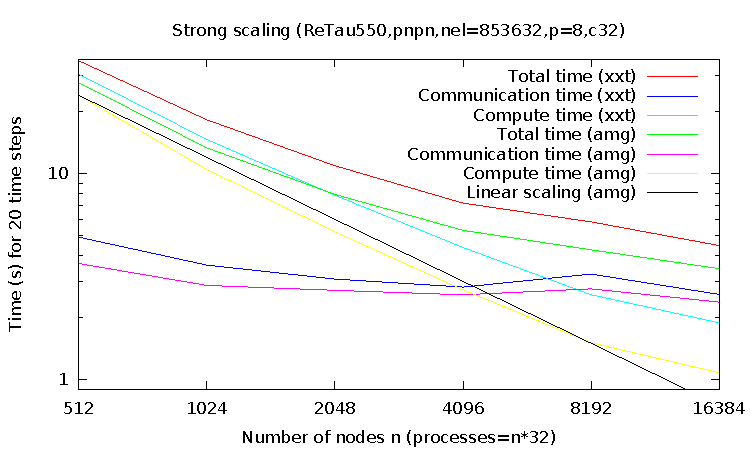
\includegraphics[width=\linewidth]{./figures/mira/scaling_ReTau550.pdf}
  }
  \subfigure[ReTau1000 Mira]{
  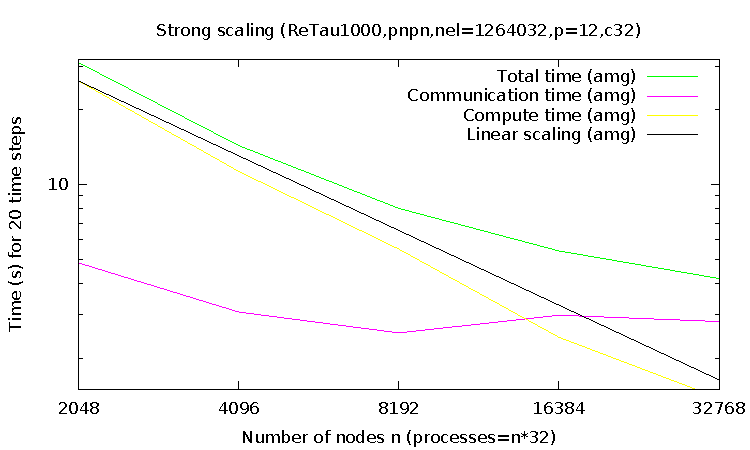
\includegraphics[width=\linewidth]{./figures/mira/scaling_ReTau1000.pdf}
  }
  \caption{BG/Q Mira}
  \label{fig:scaling_mira}
\end{figure}

\newpage

\begin{figure}
  \centering
  \subfigure[ReTau180]{
  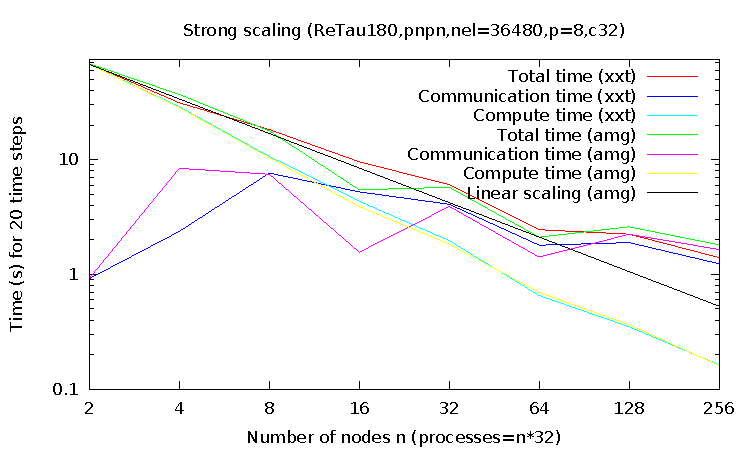
\includegraphics[width=\linewidth]{./figures/beskow/scaling_ReTau180.pdf}
  }
  \subfigure[ReTau360]{
  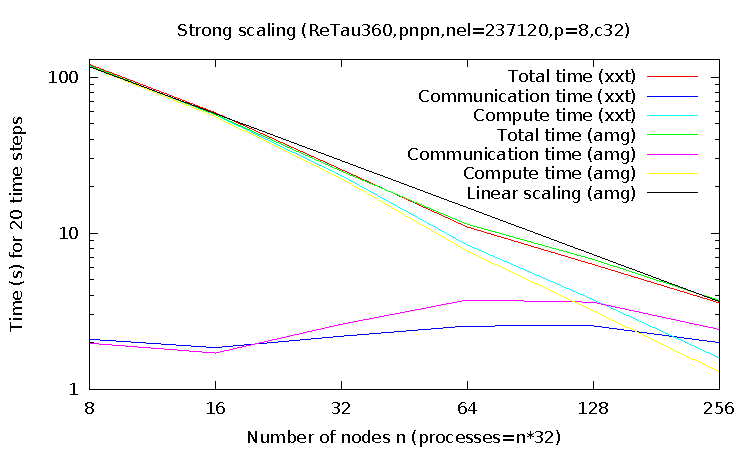
\includegraphics[width=\linewidth]{./figures/beskow/scaling_ReTau360.pdf}
  }
  \subfigure[ReTau550]{
  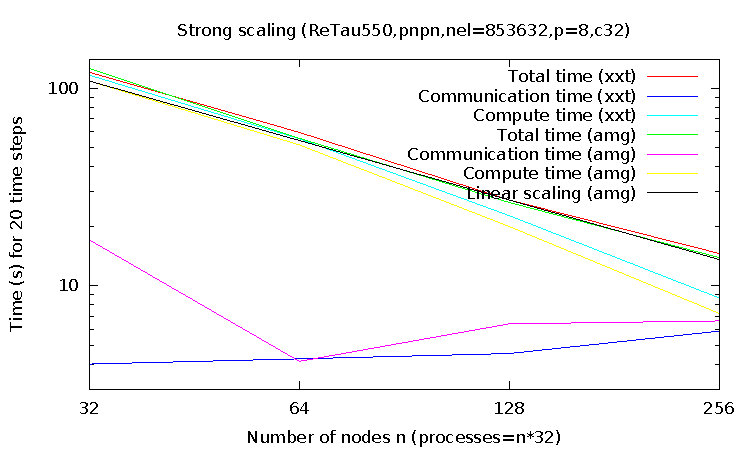
\includegraphics[width=\linewidth]{./figures/beskow/scaling_ReTau550.pdf}
  }
  \subfigure[ReTau1000]{
  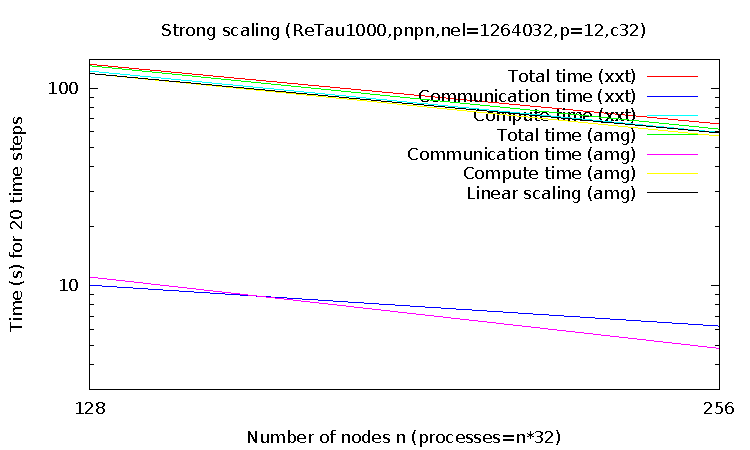
\includegraphics[width=\linewidth]{./figures/beskow/scaling_ReTau1000.pdf}
  }
\caption{Beskow}
\label{fig:scaling_beskow}
\end{figure}

\begin{figure}
  \centering
  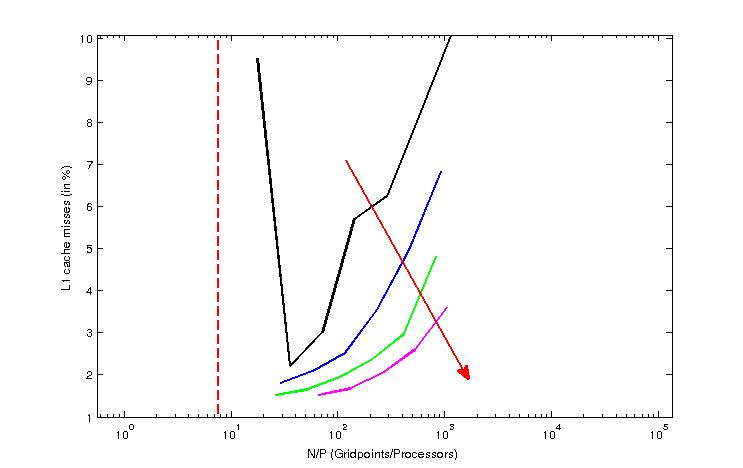
\includegraphics[width=\linewidth]{./figures/cachelines.jpg}
\end{figure}
\begin{figure}
  \centering
  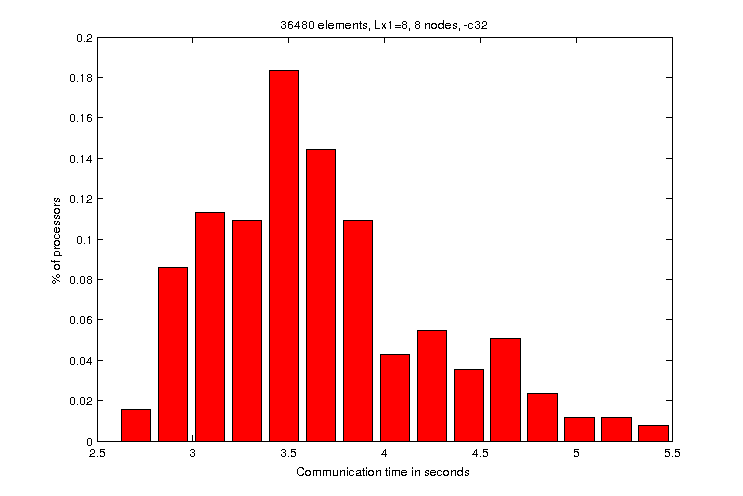
\includegraphics[width=\linewidth]{./figures/loadbalance.png}
\end{figure}
\begin{figure}
  \centering
  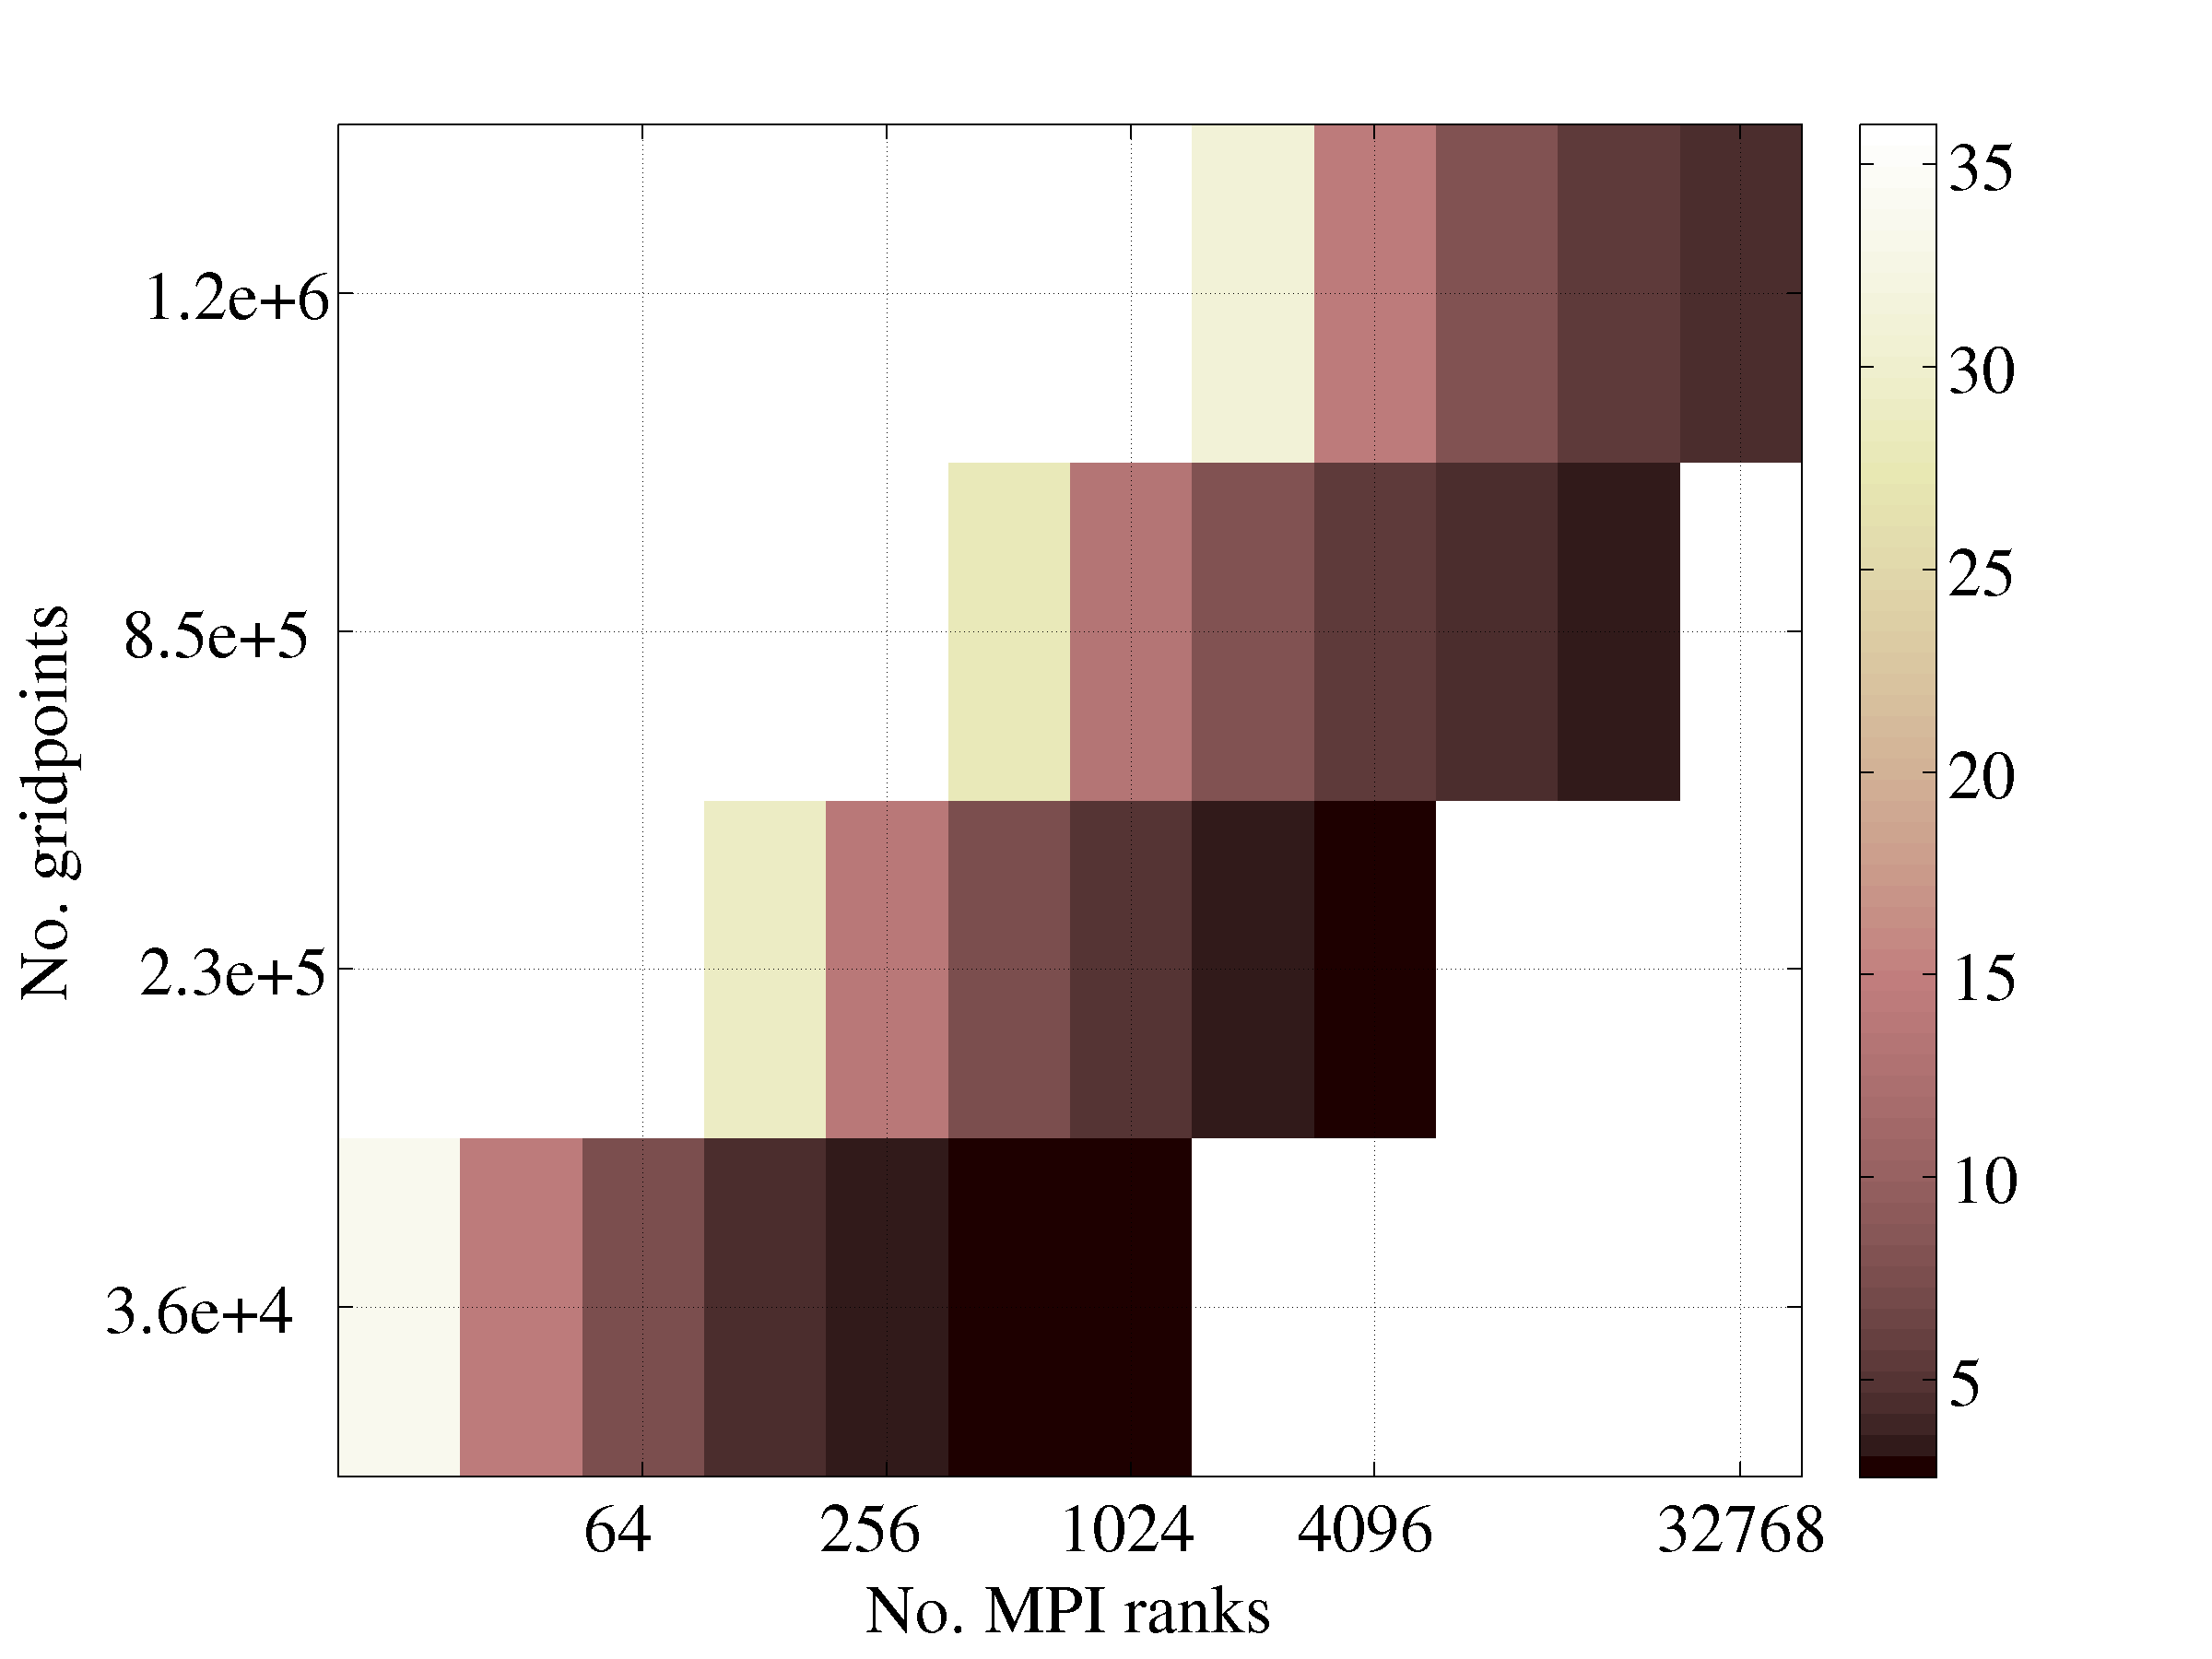
\includegraphics[width=\linewidth]{./figures/weak.png}
\end{figure}

\subsection{Weak and Strong Scaling}
With link to each subsection in \refsec{sec:abstractions}


\subsection{Communication versus Computation}
The ratio of computation and communication time $r=\frac{T_a}{T_c}$ is a key
indicator for the strong scaling limit. If communication takes longer than
computation, the code is deemed to be at the strong scaling limit where the
scaling diverges significantly from the perfect linear scaling.  

On Mira this limit has consistently been at around 





\section{Conclusions}
%\end{document}  % This is where a 'short' article might terminate

%ACKNOWLEDGMENTS are optional
\section{Acknowledgments}

%
% The following two commands are all you need in the
% initial runs of your .tex file to
% produce the bibliography for the citations in your paper.
\bibliographystyle{abbrv}
\bibliography{easc2016}  % template.bib is the name of the Bibliography in this case
% You must have a proper ".bib" file
%  and remember to run:
% latex bibtex latex latex
% to resolve all references
%
% ACM needs 'a single self-contained file'!
%
%APPENDICES are optional
%\balancecolumns
\appendix
%Appendix A
\section{Appendix A}
\label{sec:plots}
% This next section command marks the start of
% Appendix B, and does not continue the present hierarchy

%\balancecolumns % GM June 2007
% That's all folks!
Test what is wrong
\end{document}

